\documentclass[final]{beamer}
\mode<presentation>{\usetheme{I6dv}}
%\usefonttheme[onlymath]{serif}
\usefonttheme{default}

\usepackage[orientation=landscape,size=a1]{beamerposter} 
\usepackage{microtype}
\usepackage{fixltx2e}
\usepackage[english]{babel}
%\usepackage[T1]{fontenc}
\usepackage{amsmath,amsthm, amssymb, latexsym}
\usepackage{graphicx}
\usepackage{caption}
\usepackage{subcaption}


%\beamertemplategridbackground[1em]

%\usepackage{enumitem}
%\setitemize{itemsep=.5em}
%\setlength{\itemsep}{5em}

\begin{document}
\begin{frame}{ }
    \begin{columns}[t]
        \begin{column}{.26\linewidth}

            \begin{block}{Introduction}
                \begin{itemize}
                    \itemsep.4em
                    \item Traffic congestion is currently a major issue for transportation planning
                    \item A transportation forecasting model has been built to predict future traffic and reduce congestion
                    \item The \alert{Traffic Assignment (TA)} problem is part of the model which deals with \alert{selecting the shortest path} for travellers in the network to \alert{minimise} their \alert{travel times}
                \item \alert{Goal}: find a faster algorithm to solve the shortest path problem in the traffic assignment problem
            \end{itemize}
        \end{block}

        \begin{block}{Traffic assignment}
            \begin{itemize}
                \itemsep.4em
                    %\item \alert{Traffic Assignment (TA)} deals with selection of \alert{shortest path} for travellers in the network to \alert{minimise} their \alert{travel times}
                \item TA is a non-linear problem, where travel times increase dramatically when congestion occurs
                \item An \alert{iterative} algorithm called \alert{Path Equilibration (PE)} is used to solve TA
                \item PE requires \alert{millions of shortest paths} to be found
                \item Solving the shortest path problem faster can speed up TA and benefit transportation modelling greatly
            \end{itemize}
        \end{block}

        \begin{block}{Shortest path algorithms}
            \begin{itemize}
                \itemsep.4em
                \item A shortest path algorithm finds a path between origins and destinations with the least travel distance or time in a network
                \item The algorithm searches nodes in the network in some order until the destination is found
               \item A \alert{priority queue} is needed to store the searched nodes in some order so the next location to search can be found easily
         %       \item A data structure called \alert{priority queue} is used to store and extract the next node to search efficiently
                \item Performance of PE is affected by different shortest path algorithms and priority queue implementations 
            \end{itemize}
        \end{block}

        \begin{block}{Avoiding shortest paths}
            \begin{itemize}
                \itemsep.4em
                \item In PE, \alert{some shortest path calculations can be avoided} between iterations to speed up the overall performance
                \item The shortest path from the previous iteration can be \alert{re-used} to \alert{avoid} the calculation in the current iteration
                \item The first strategy is to \alert{avoid the next few iterations} if the shortest paths of the previous two iterations are identical
                \item The second strategy is to \alert{randomly avoid} the next shortest path calculation in the hope that the shortest path of previous and current iteration are identical
            \end{itemize}
        \end{block}

    \end{column}
    \begin{column}{.4\linewidth}
        \begin{block}{Search areas of shortest path algorithms \vspace{-.2em}}
            \begin{itemize}
                \itemsep.4em
                \item The performance of shortest path algorithms is heavily dependent on the search areas
                \item Computational time can be sped up if a smaller area is searched 
                \item The following figures demonstrate search areas of the implemented shortest path algorithms on part of the Chicago regional network, which has $546$ nodes and $2{,}950$ arcs
            \end{itemize}
            \vspace{1em}
            \begin{figure}
                \centering
                \begin{subfigure}{.5\linewidth}
                    \centering
                    {\bfseries Dijkstra's algorithm }
                    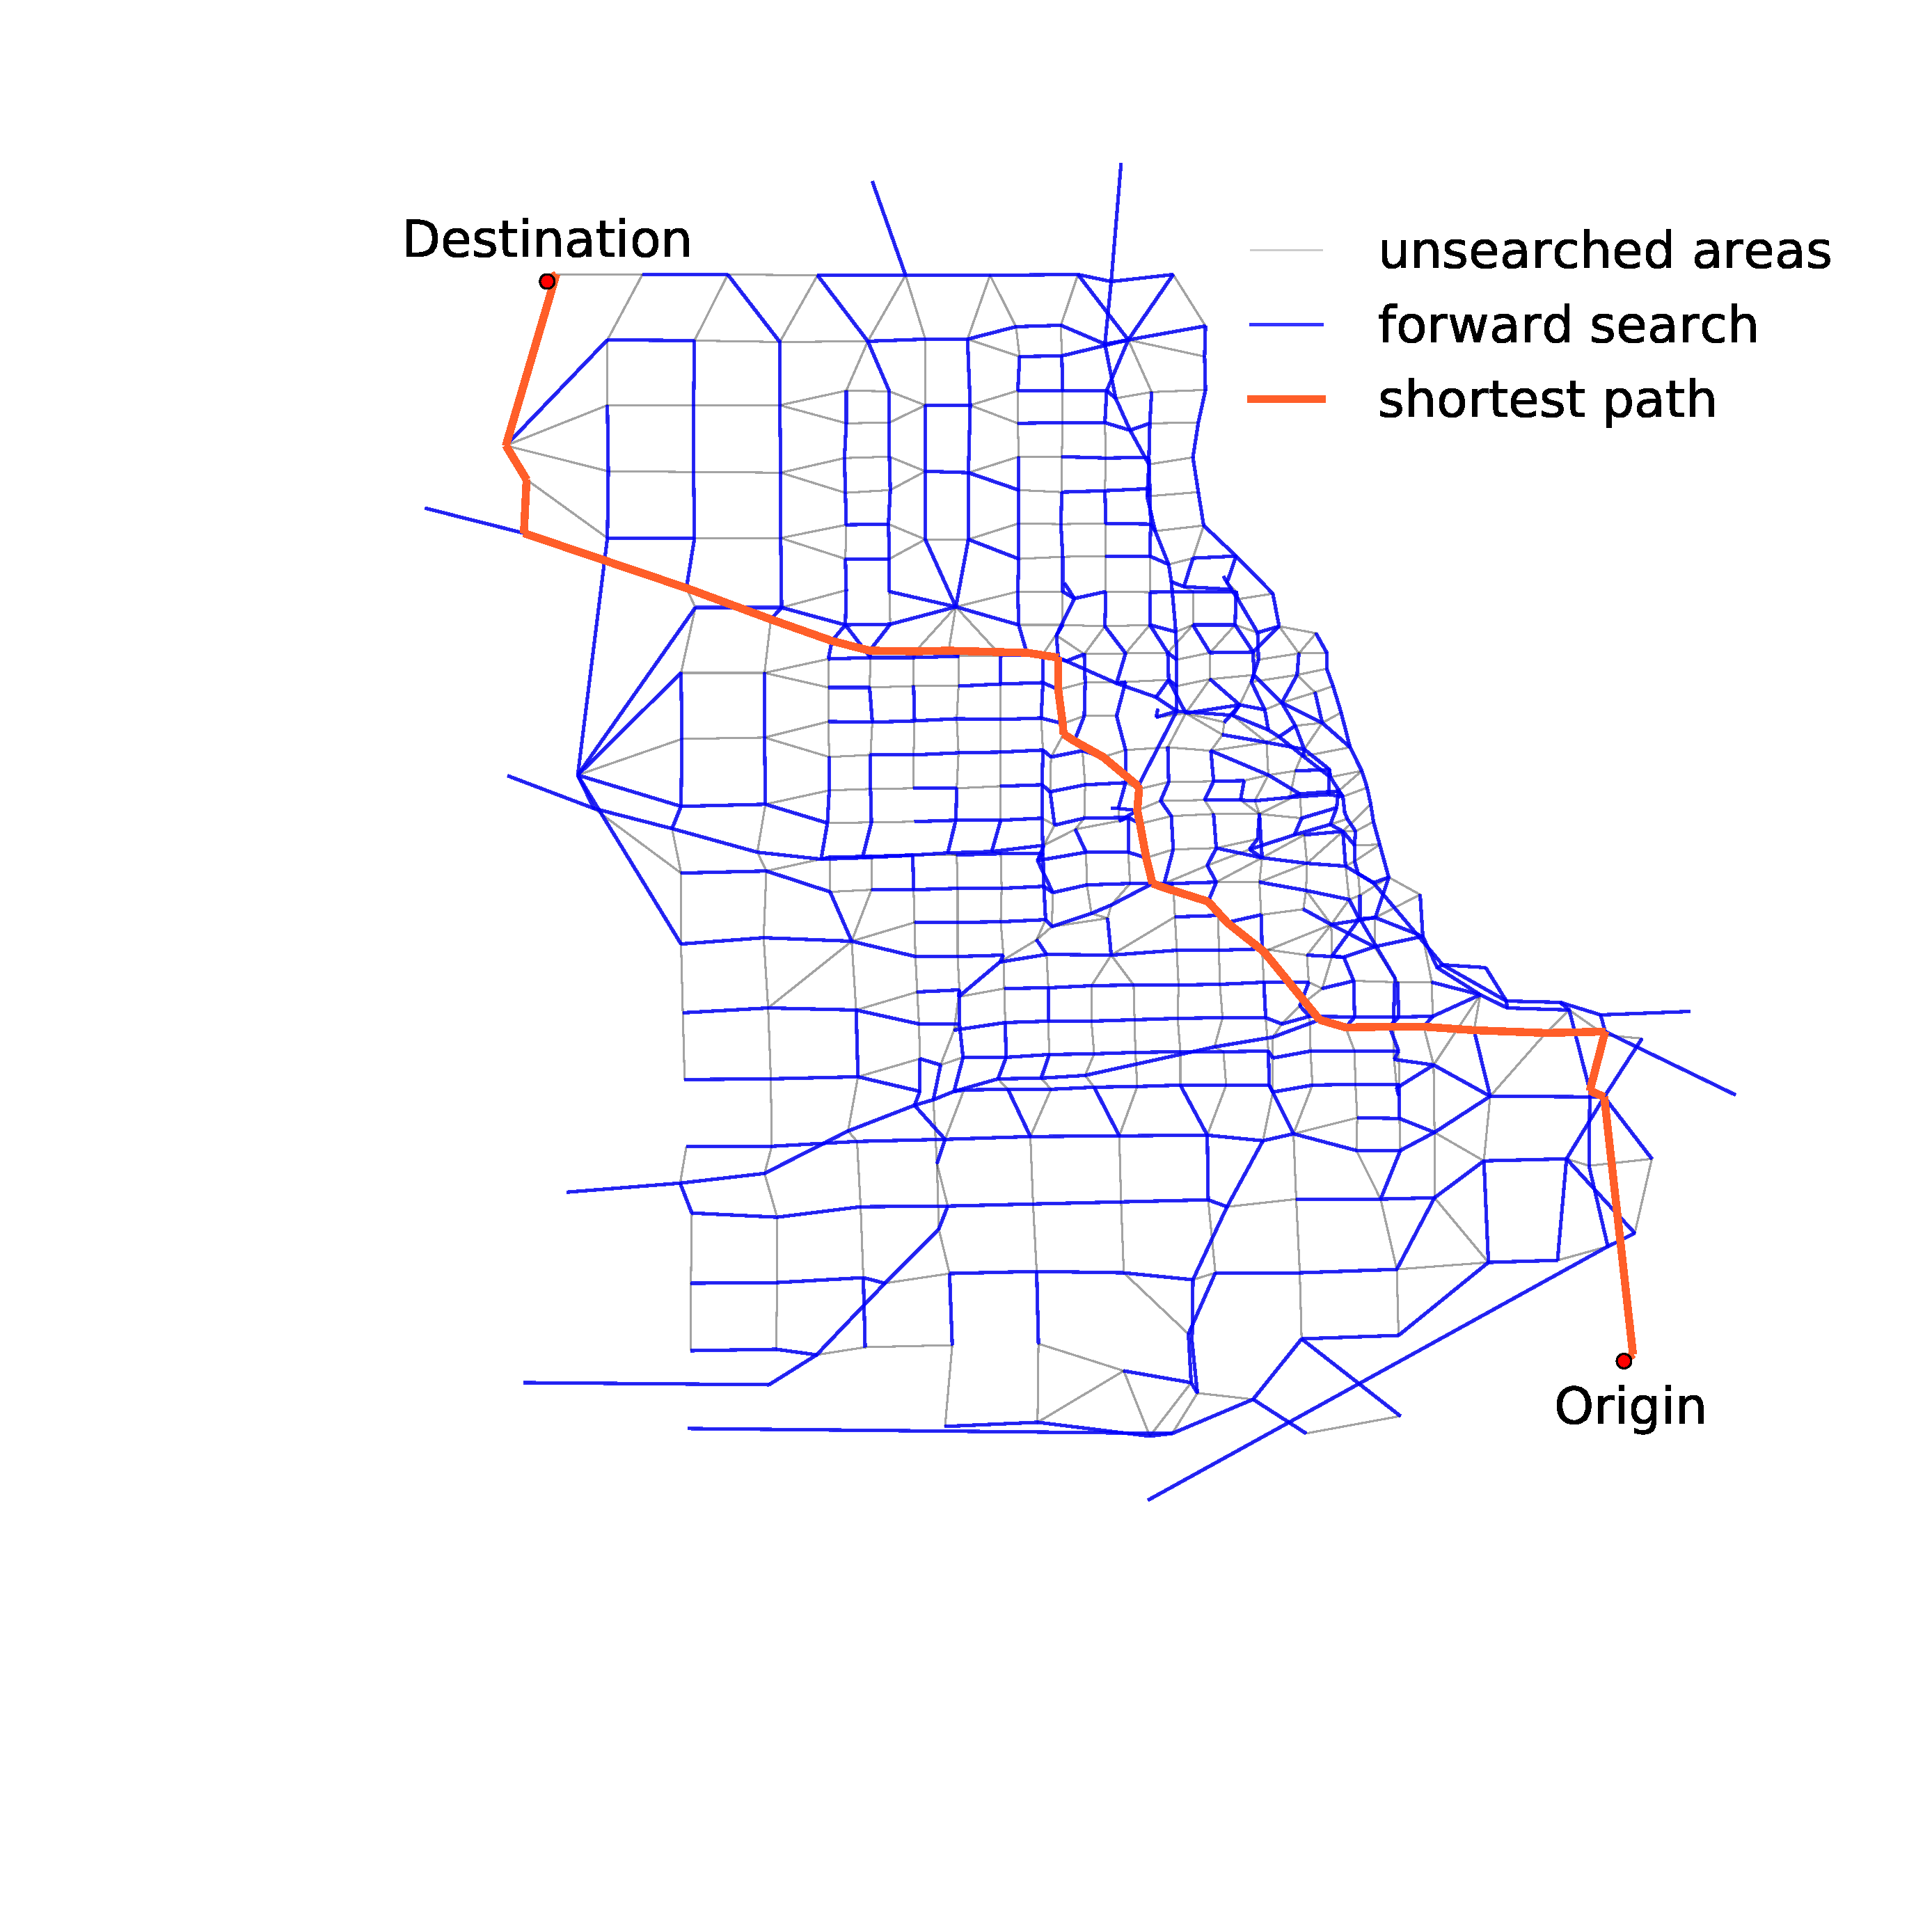
\includegraphics[width=\linewidth,trim=120px 280px 48px 60px,clip]{img/dijkstra}
                    \begin{itemize}
                            \centering
                        \item search the entire network
                    \end{itemize}
                \end{subfigure}%
                \begin{subfigure}{.5\linewidth}
                    \vspace{.1em}
                    \centering
                    {\bfseries Bidirectional Dijkstra's algorithm}
                    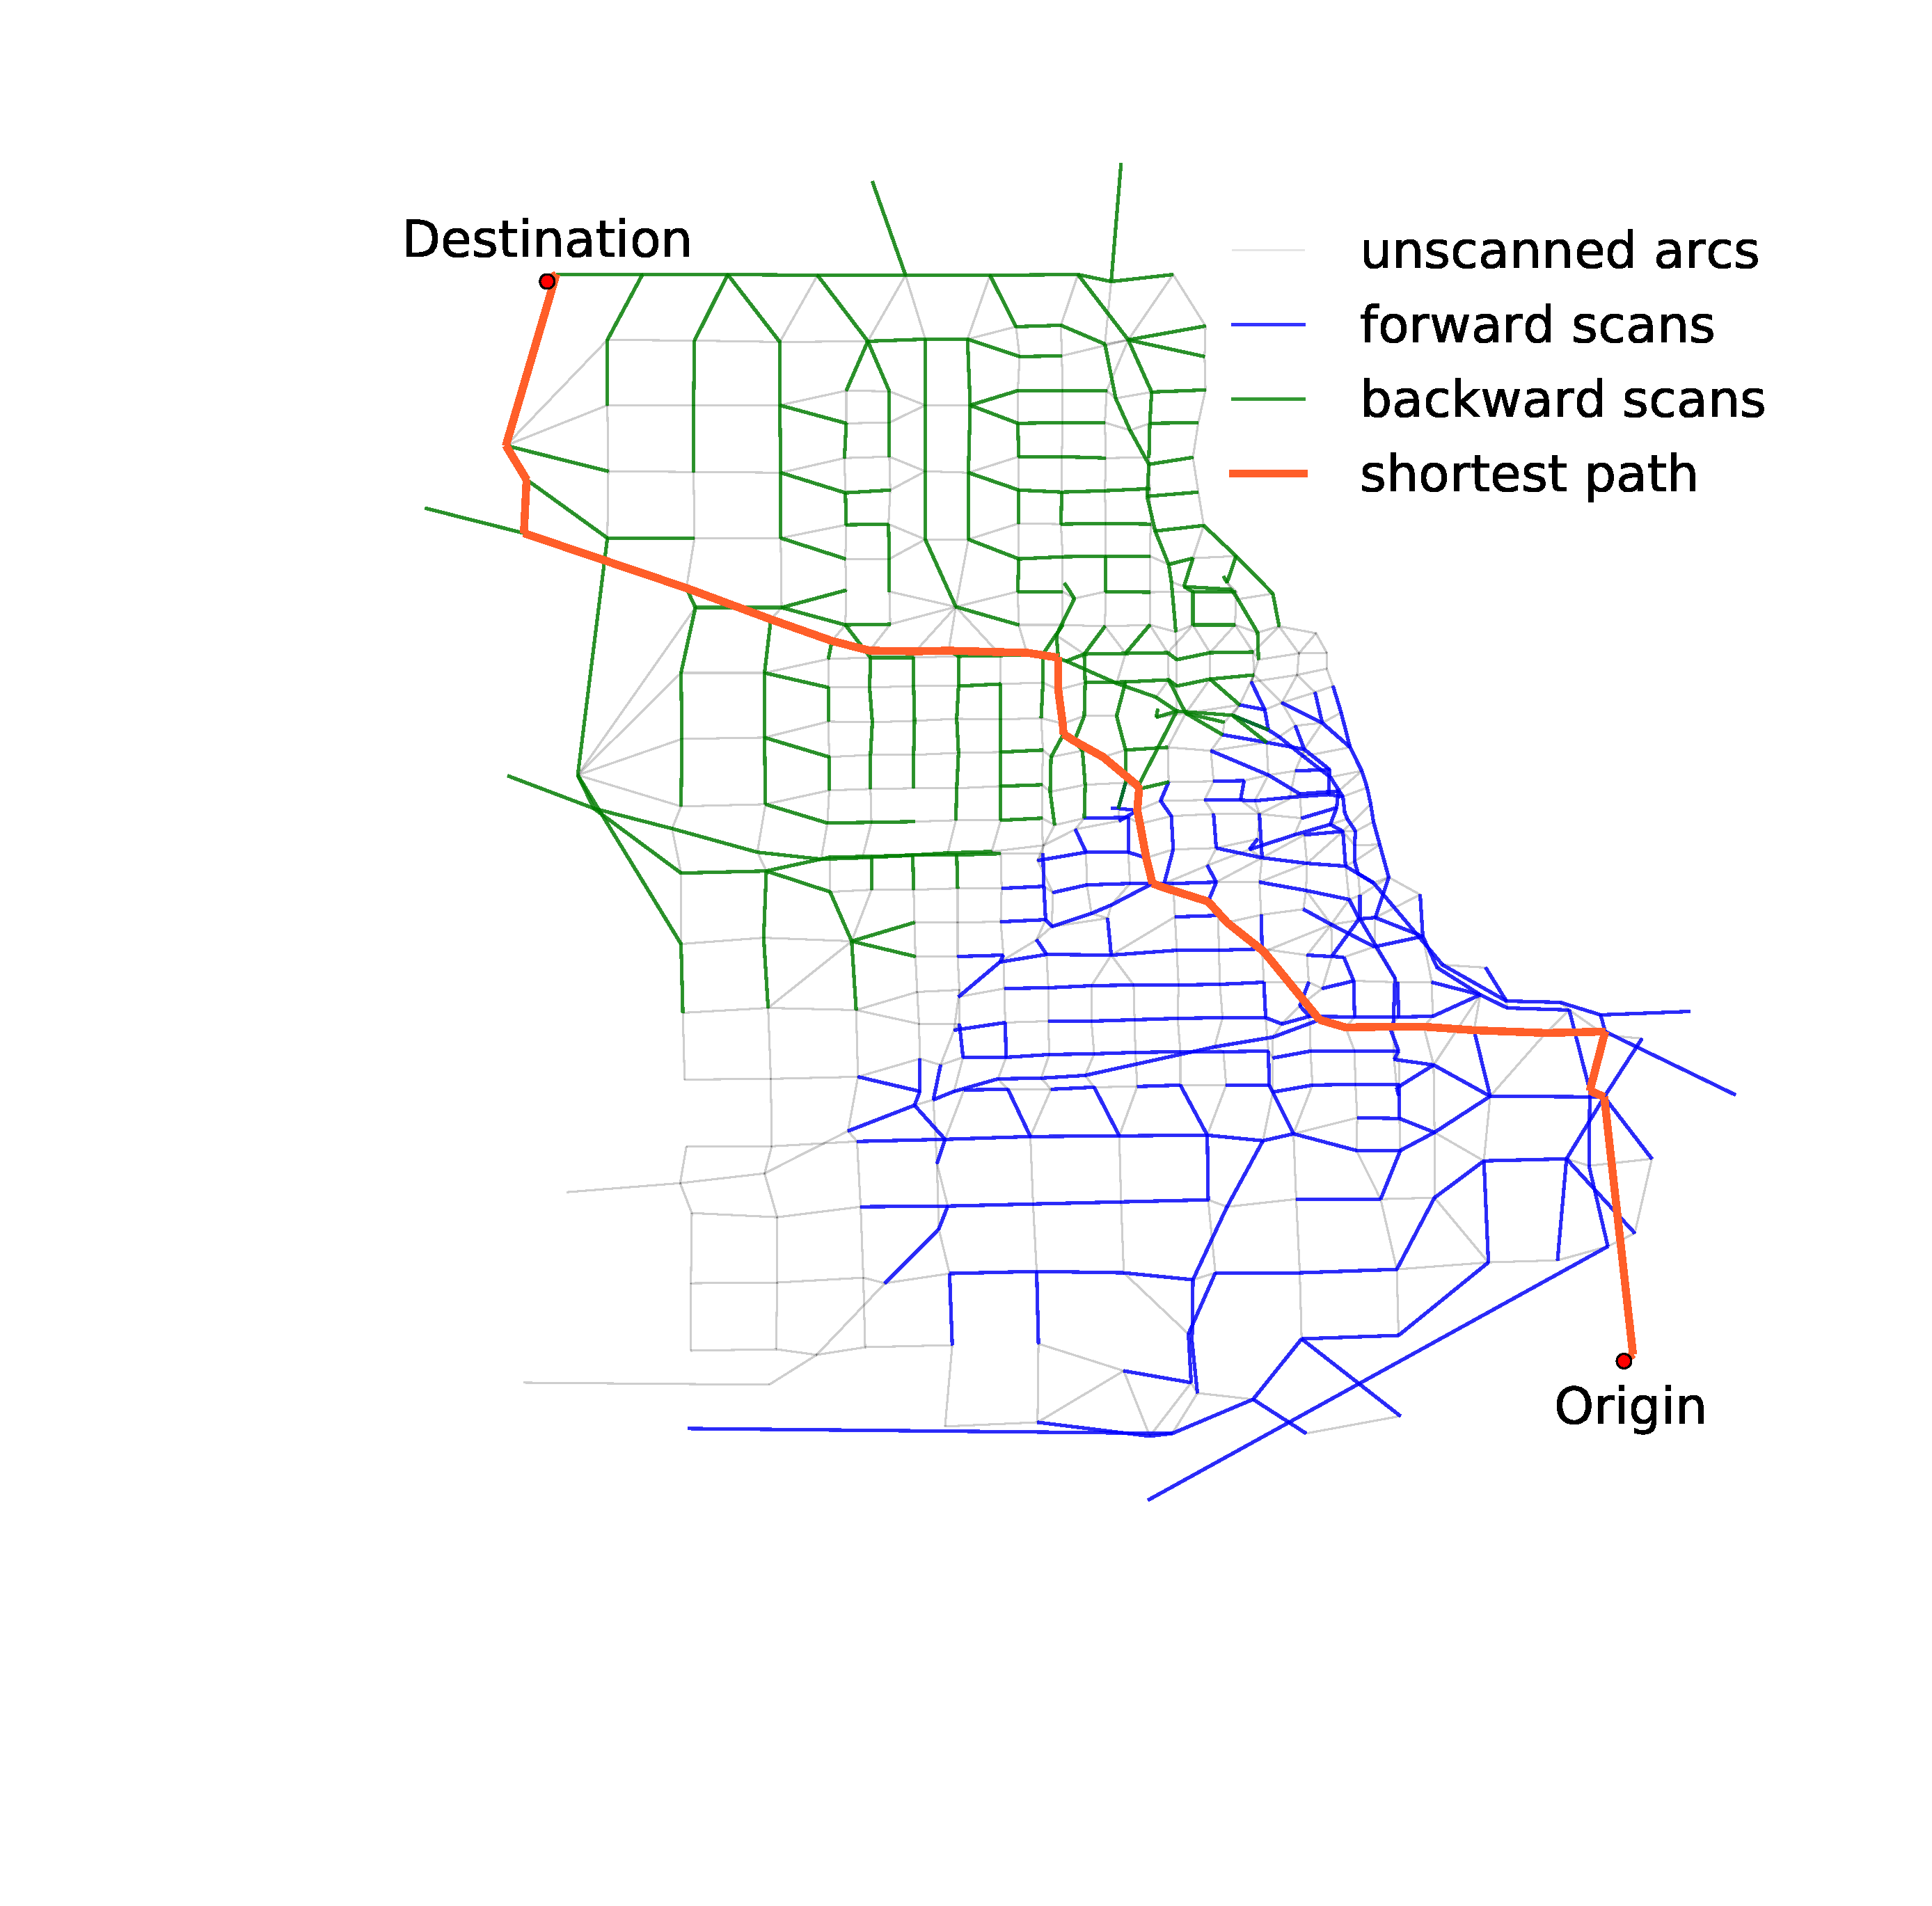
\includegraphics[width=\linewidth,trim=120px 280px 48px 60px,clip]{img/dijkstra_bidirect}
                    \begin{itemize}
                            \centering
                        \item alternatively search from both ends
                    \end{itemize}
                \end{subfigure}
                \begin{subfigure}{.5\linewidth}
                    \centering
                    {\bfseries A* Search}
                    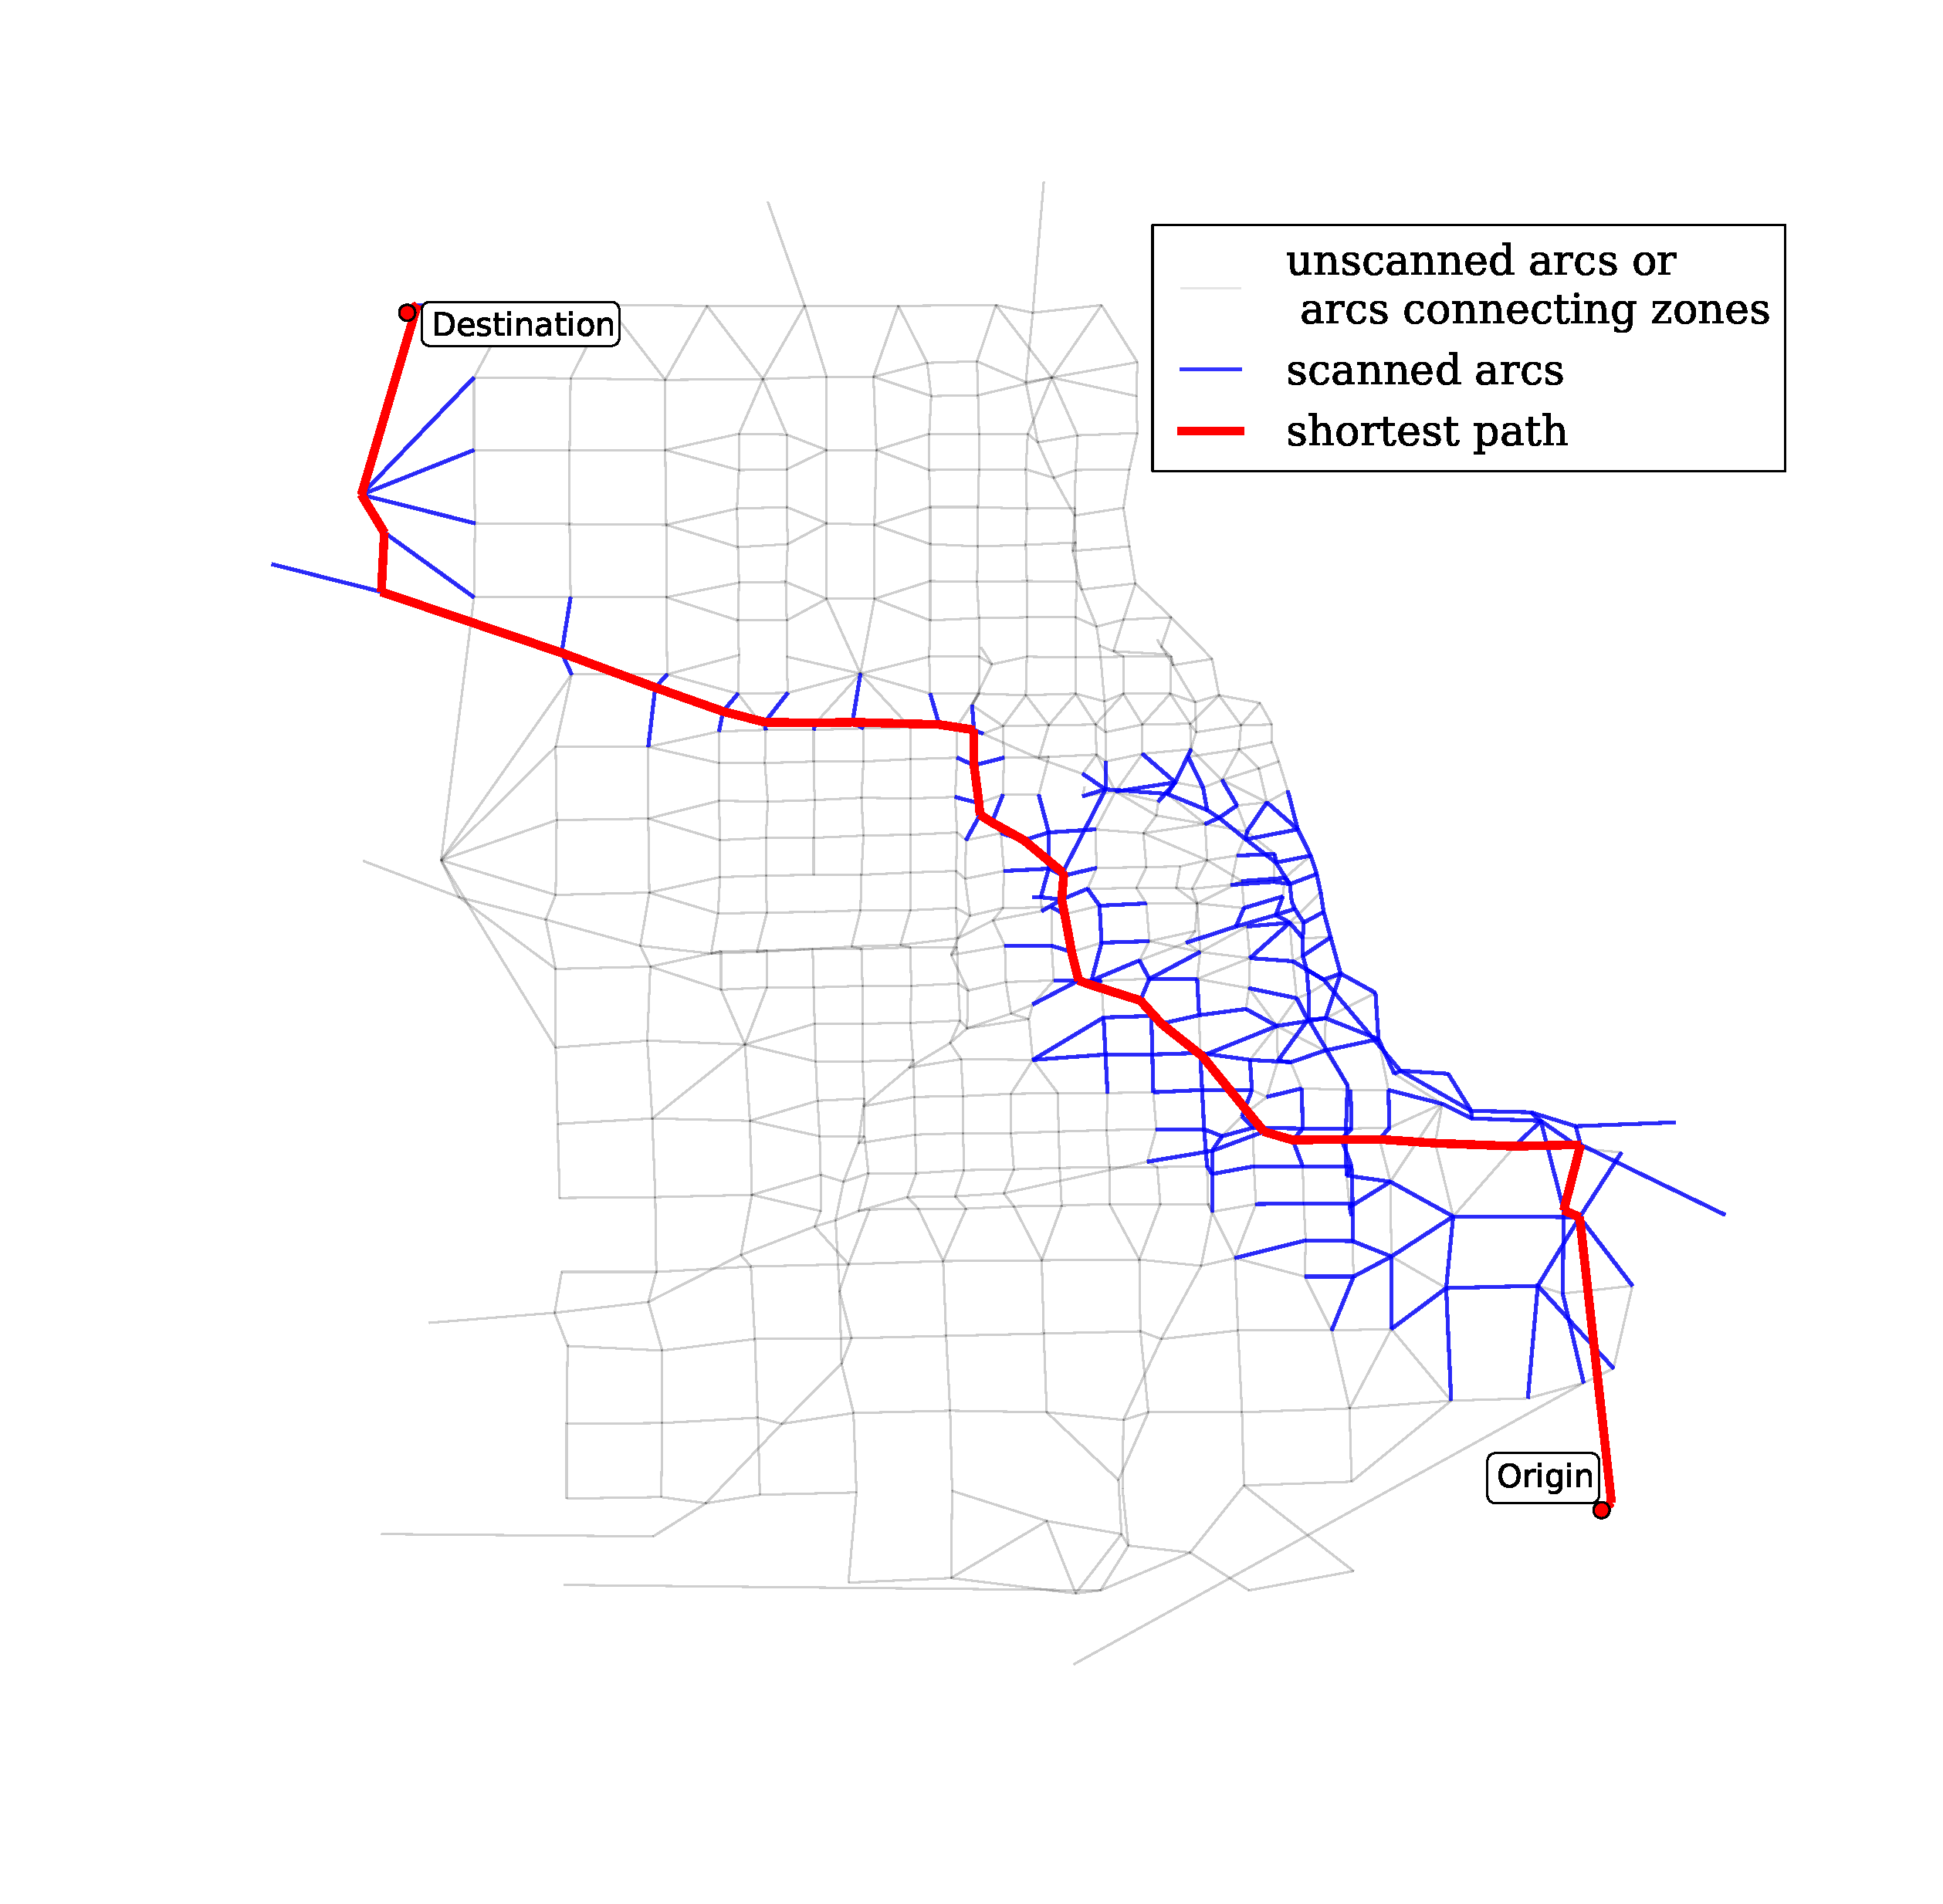
\includegraphics[width=\linewidth,trim=120px 280px 48px 60px,clip]{img/astar}
                    \begin{itemize}
                            \centering
                        \item search along the expected shortest path
                    \end{itemize}
                \end{subfigure}%
                \begin{subfigure}{.5\linewidth}
                    \vspace{1.3em}
                    \centering
                    {\bfseries Bidirectional A* Search}
                    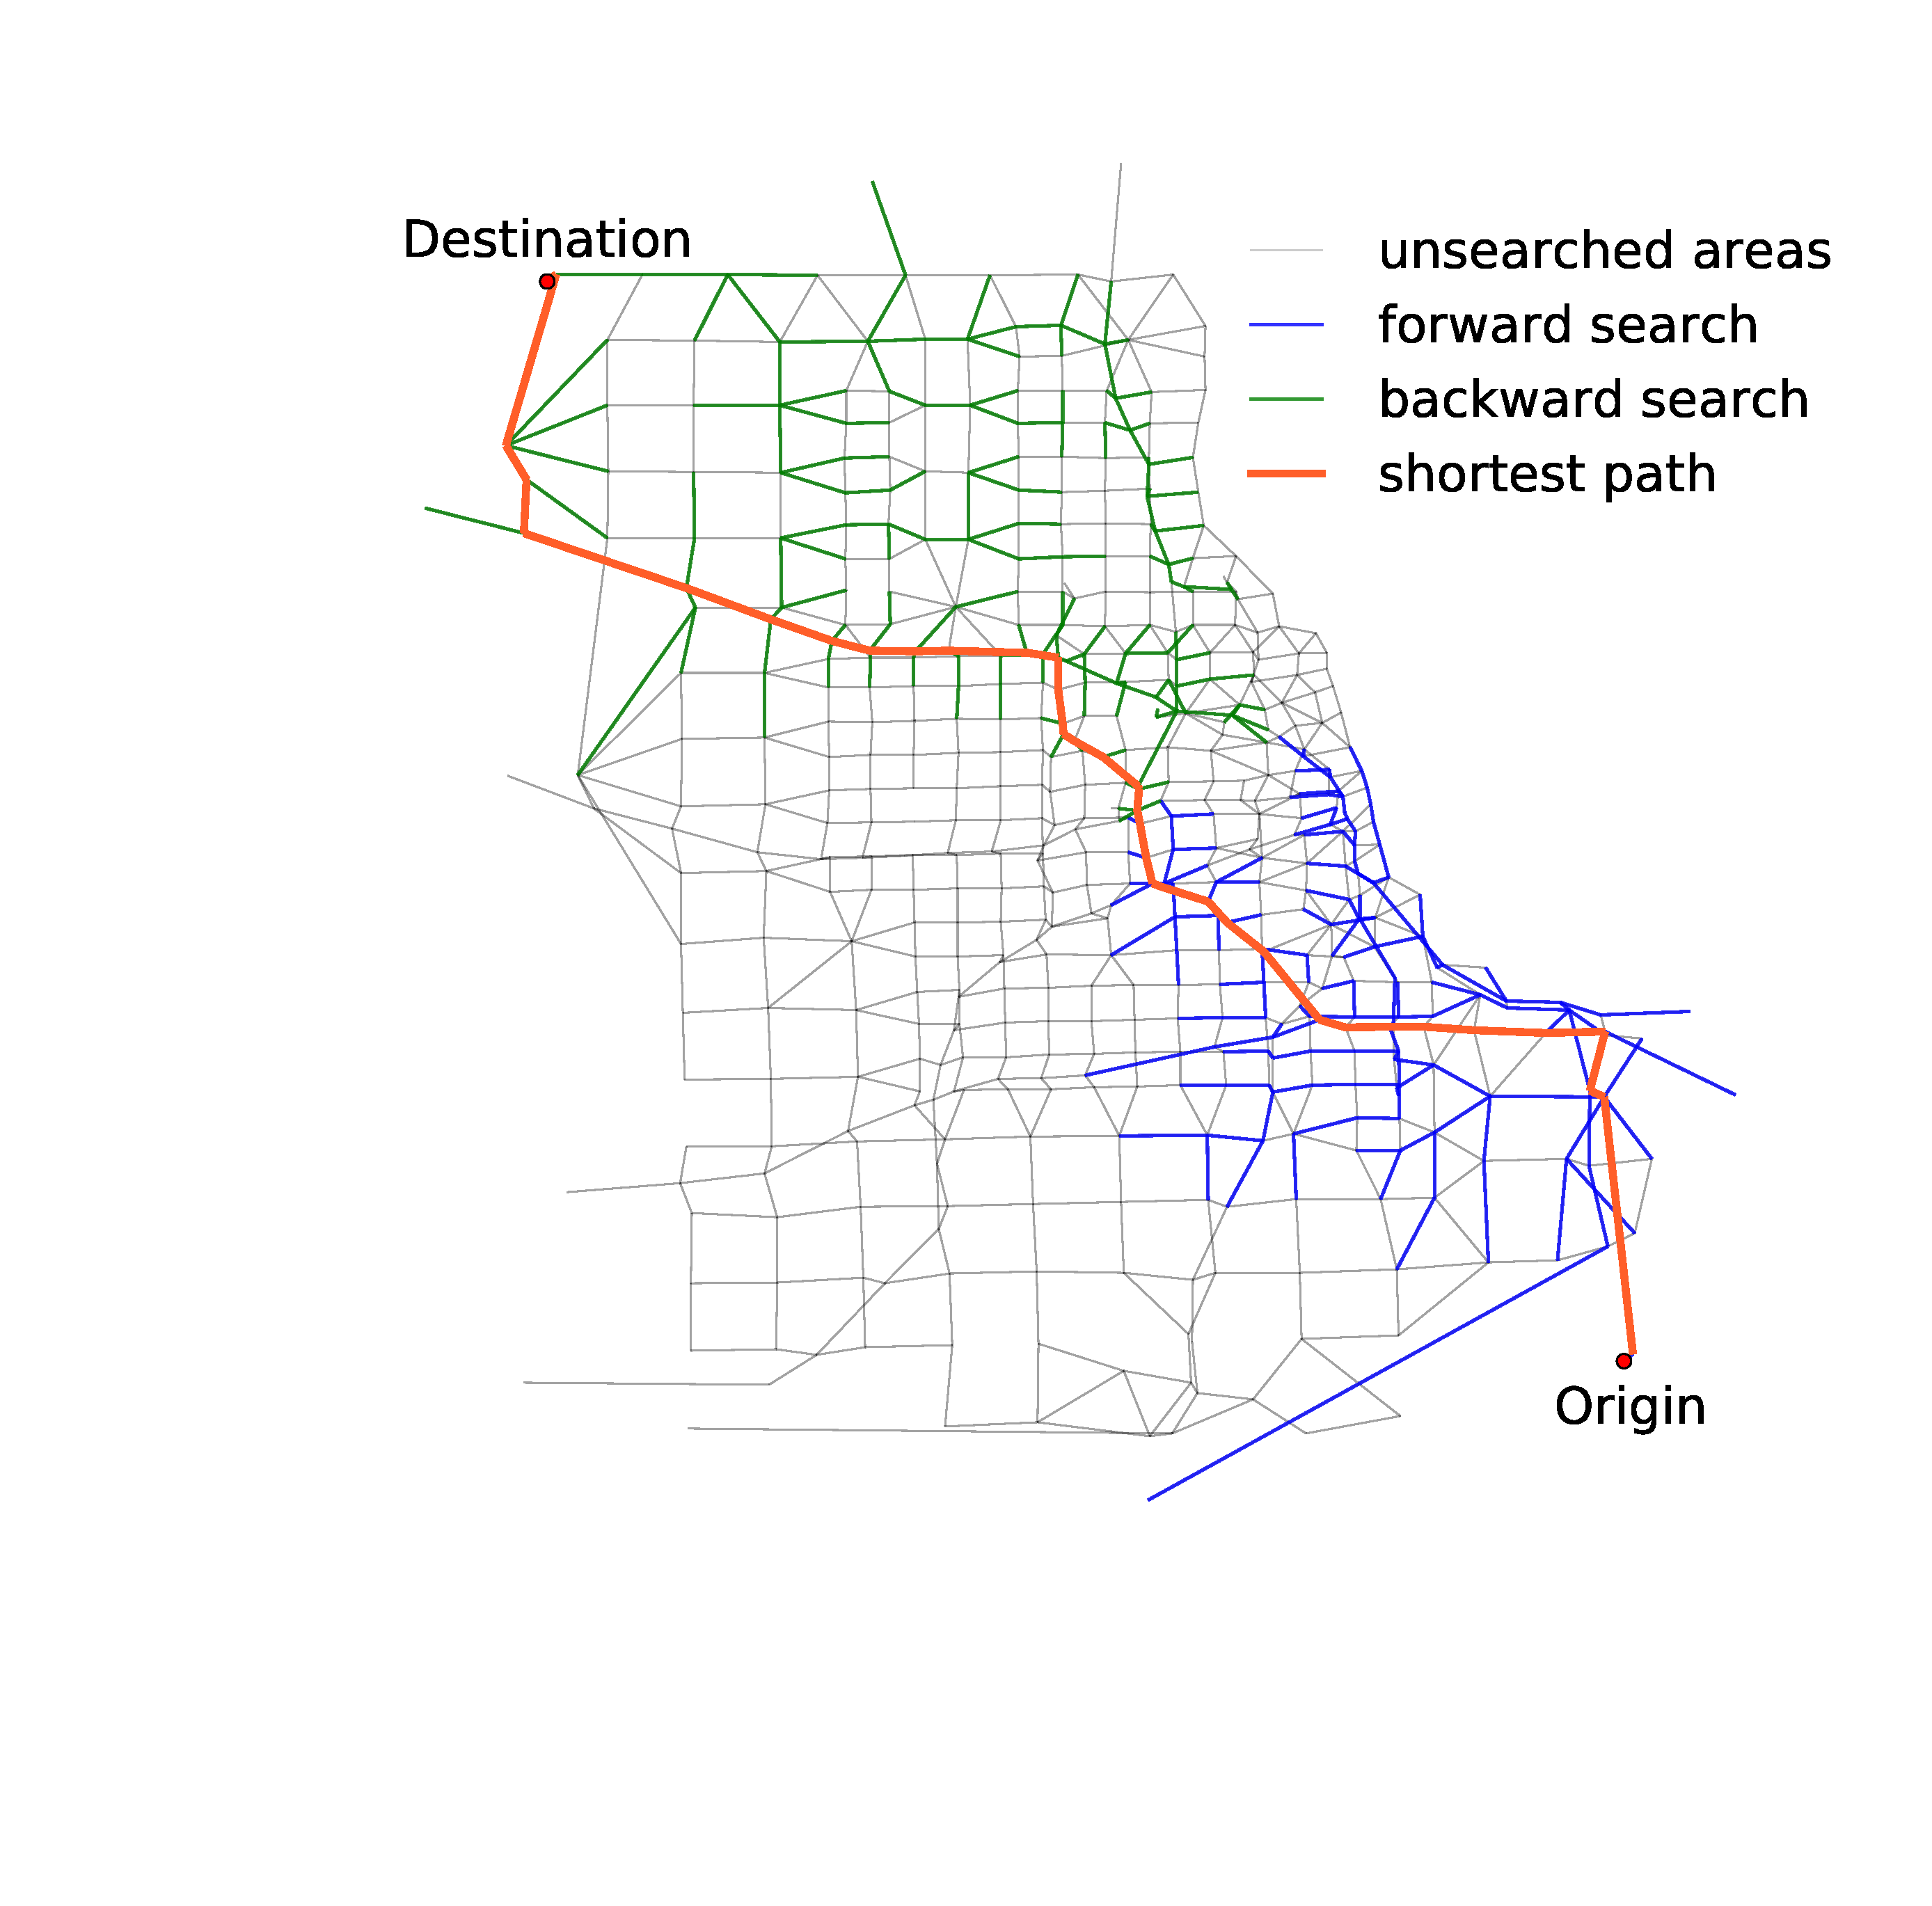
\includegraphics[width=\linewidth,trim=120px 280px 48px 60px,clip]{img/astar_bidirect}
                    \begin{itemize}
                            \centering
                        \item alternatively search along the expected shortest path from both ends
                    \end{itemize}
                \end{subfigure}
            \end{figure}
            \begin{itemize}
                \itemsep.4em
                \item Dijkstra's algorithm searches the largest area
                \item Bidirectional Dijkstra's algorithm performs less searches 
                \item \alert{A* search searches the smallest area}
                \item Bidirectional A* search searches more than unidirectional A*
            \end{itemize}
        \end{block}

    \end{column}
    \begin{column}{.26\linewidth}
        \begin{block}{Results}
            \begin{itemize}
                \itemsep.4em
                \item 8 different priority queues were tested, 4 shortest path algorithms were implemented and 2 strategies for avoiding shortest path calculation in PE were tested on the same part of the Chicago regional network
            \end{itemize}
            \begin{figure}
                \centering
                {\bfseries \qquad Run times of Dijkstra's algorithm\\ \qquad using different priority queues}
                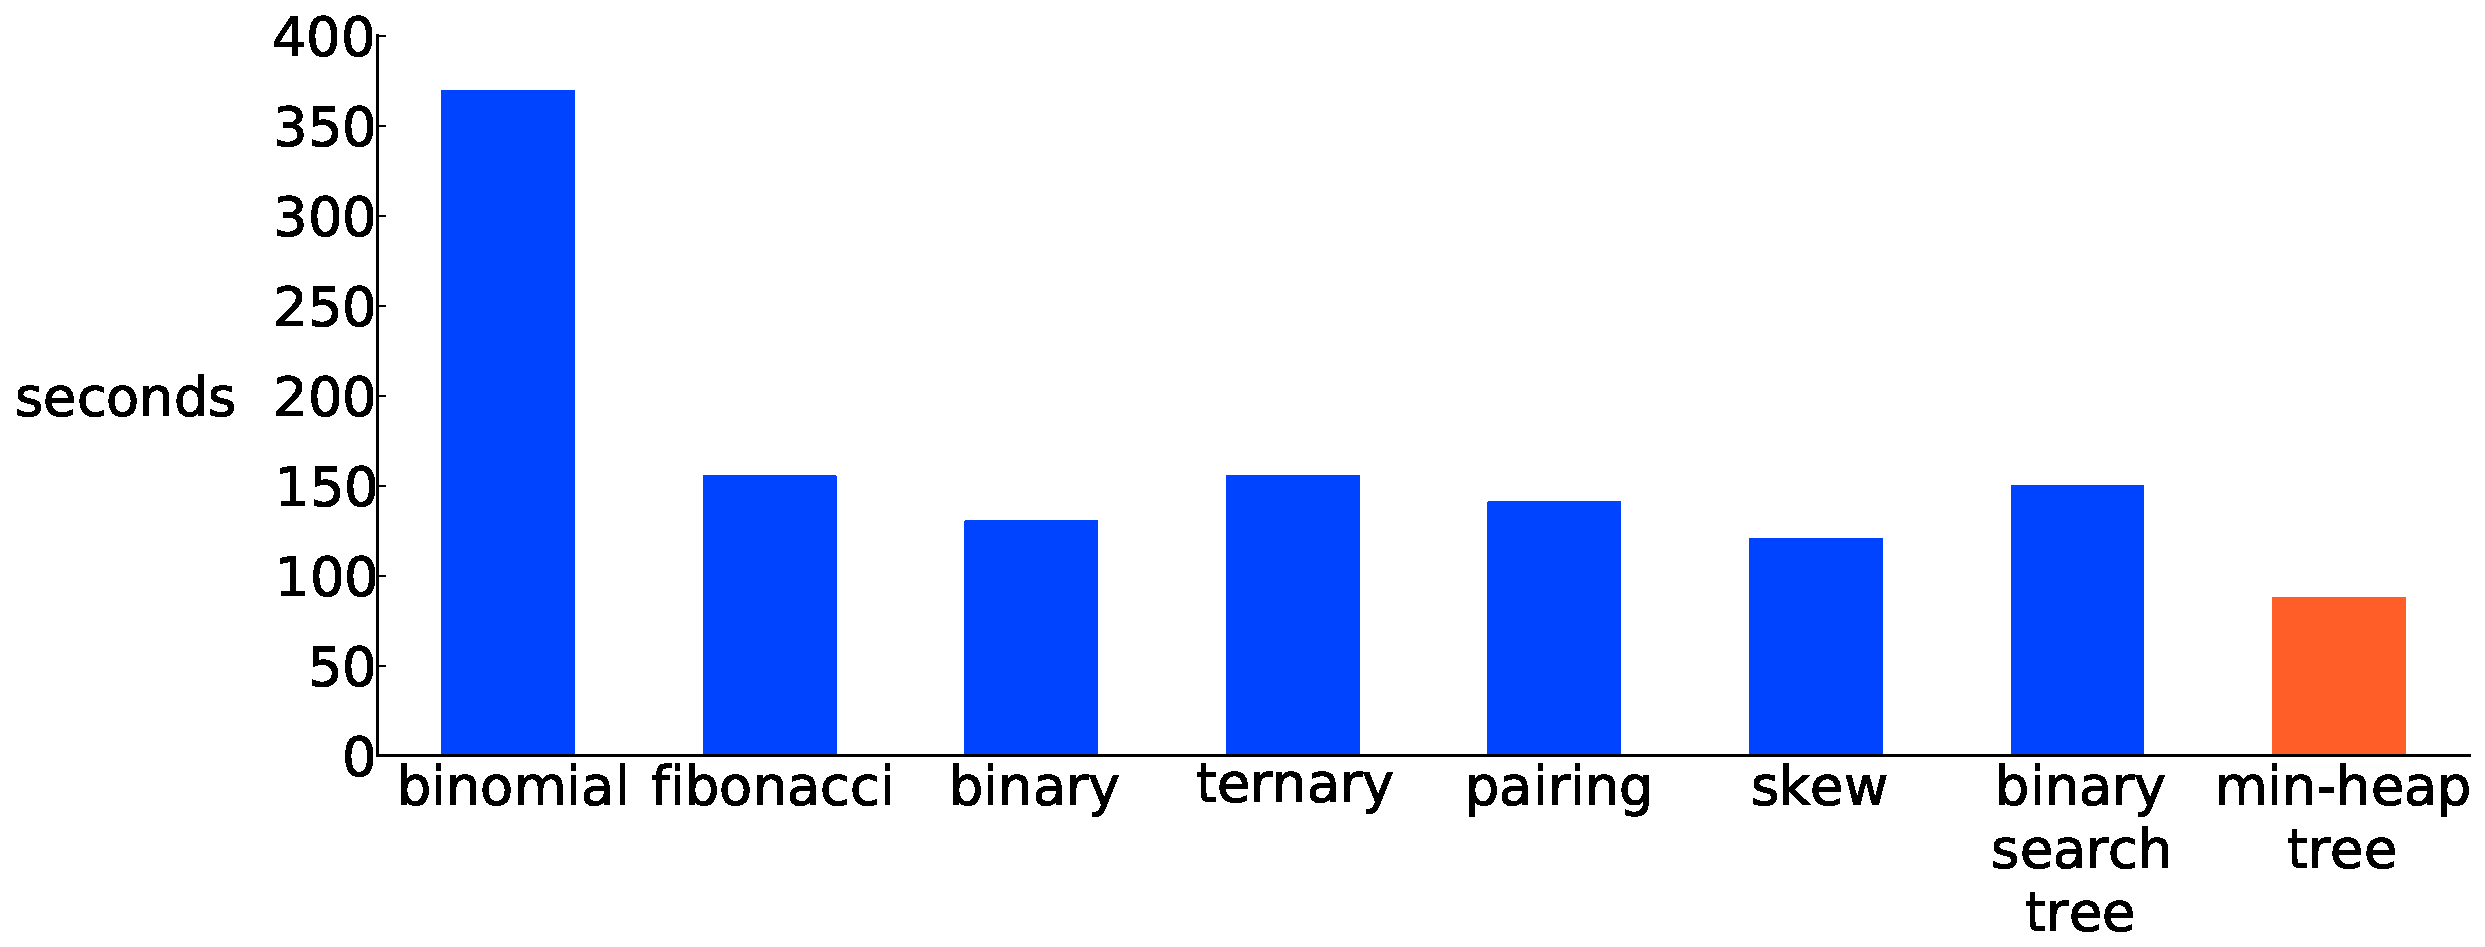
\includegraphics[width=\linewidth]{img/pq_runtime}
            \end{figure}
            \begin{figure}
                \centering
                {\bfseries \qquad Run times of shortest path algorithms\\ using binary min-heap tree}
                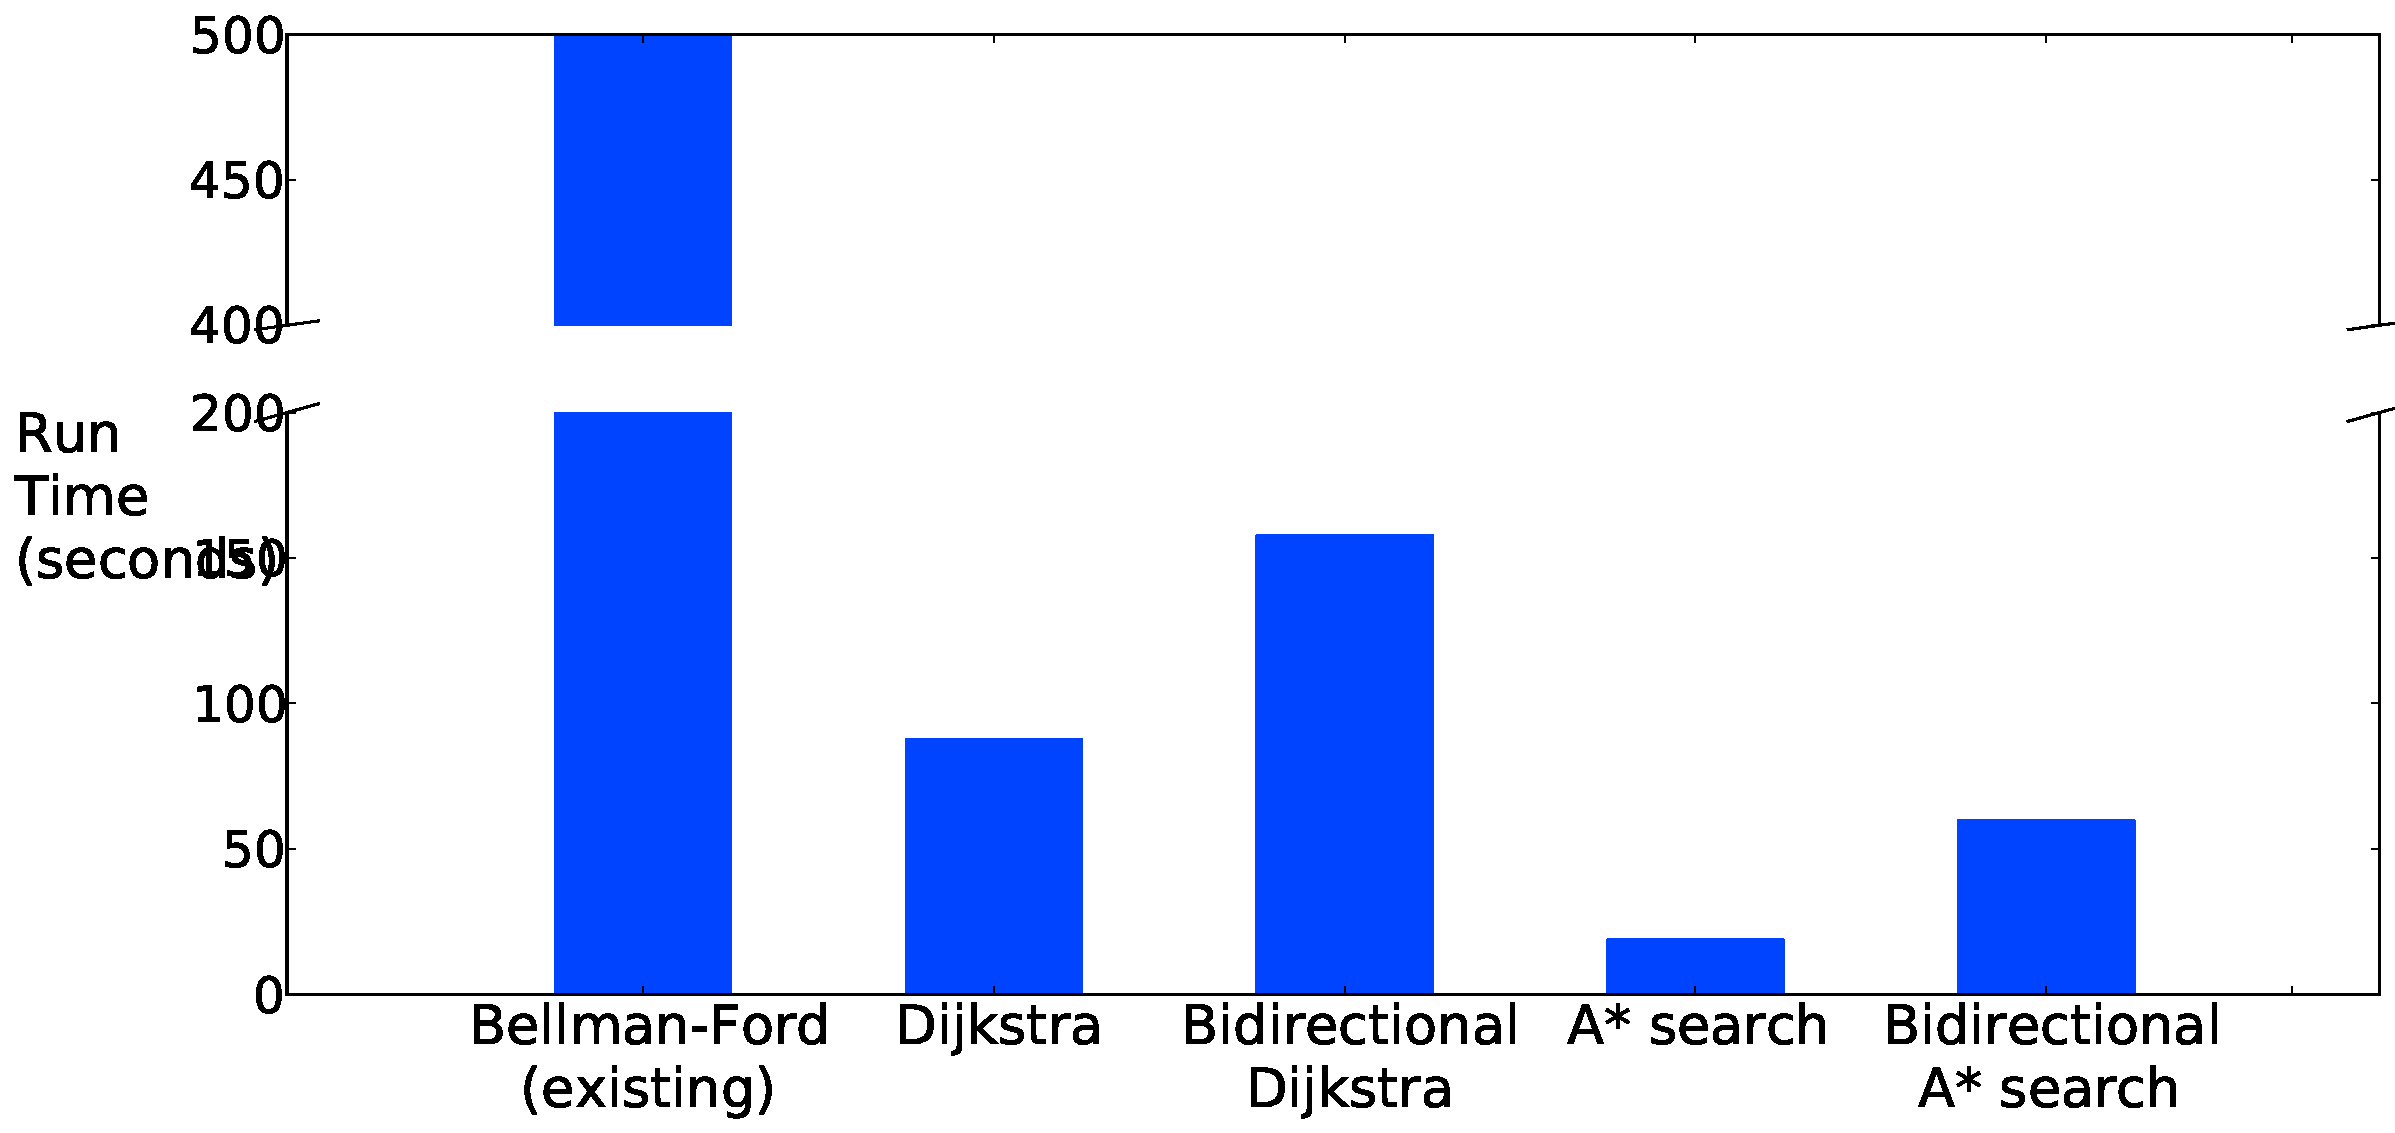
\includegraphics[width=\linewidth]{img/runtime}
            \end{figure}
            \begin{figure}
                \centering
                {\bfseries \qquad Run times of A* search using avoiding\\ \qquad shortest path calculation strategies}
                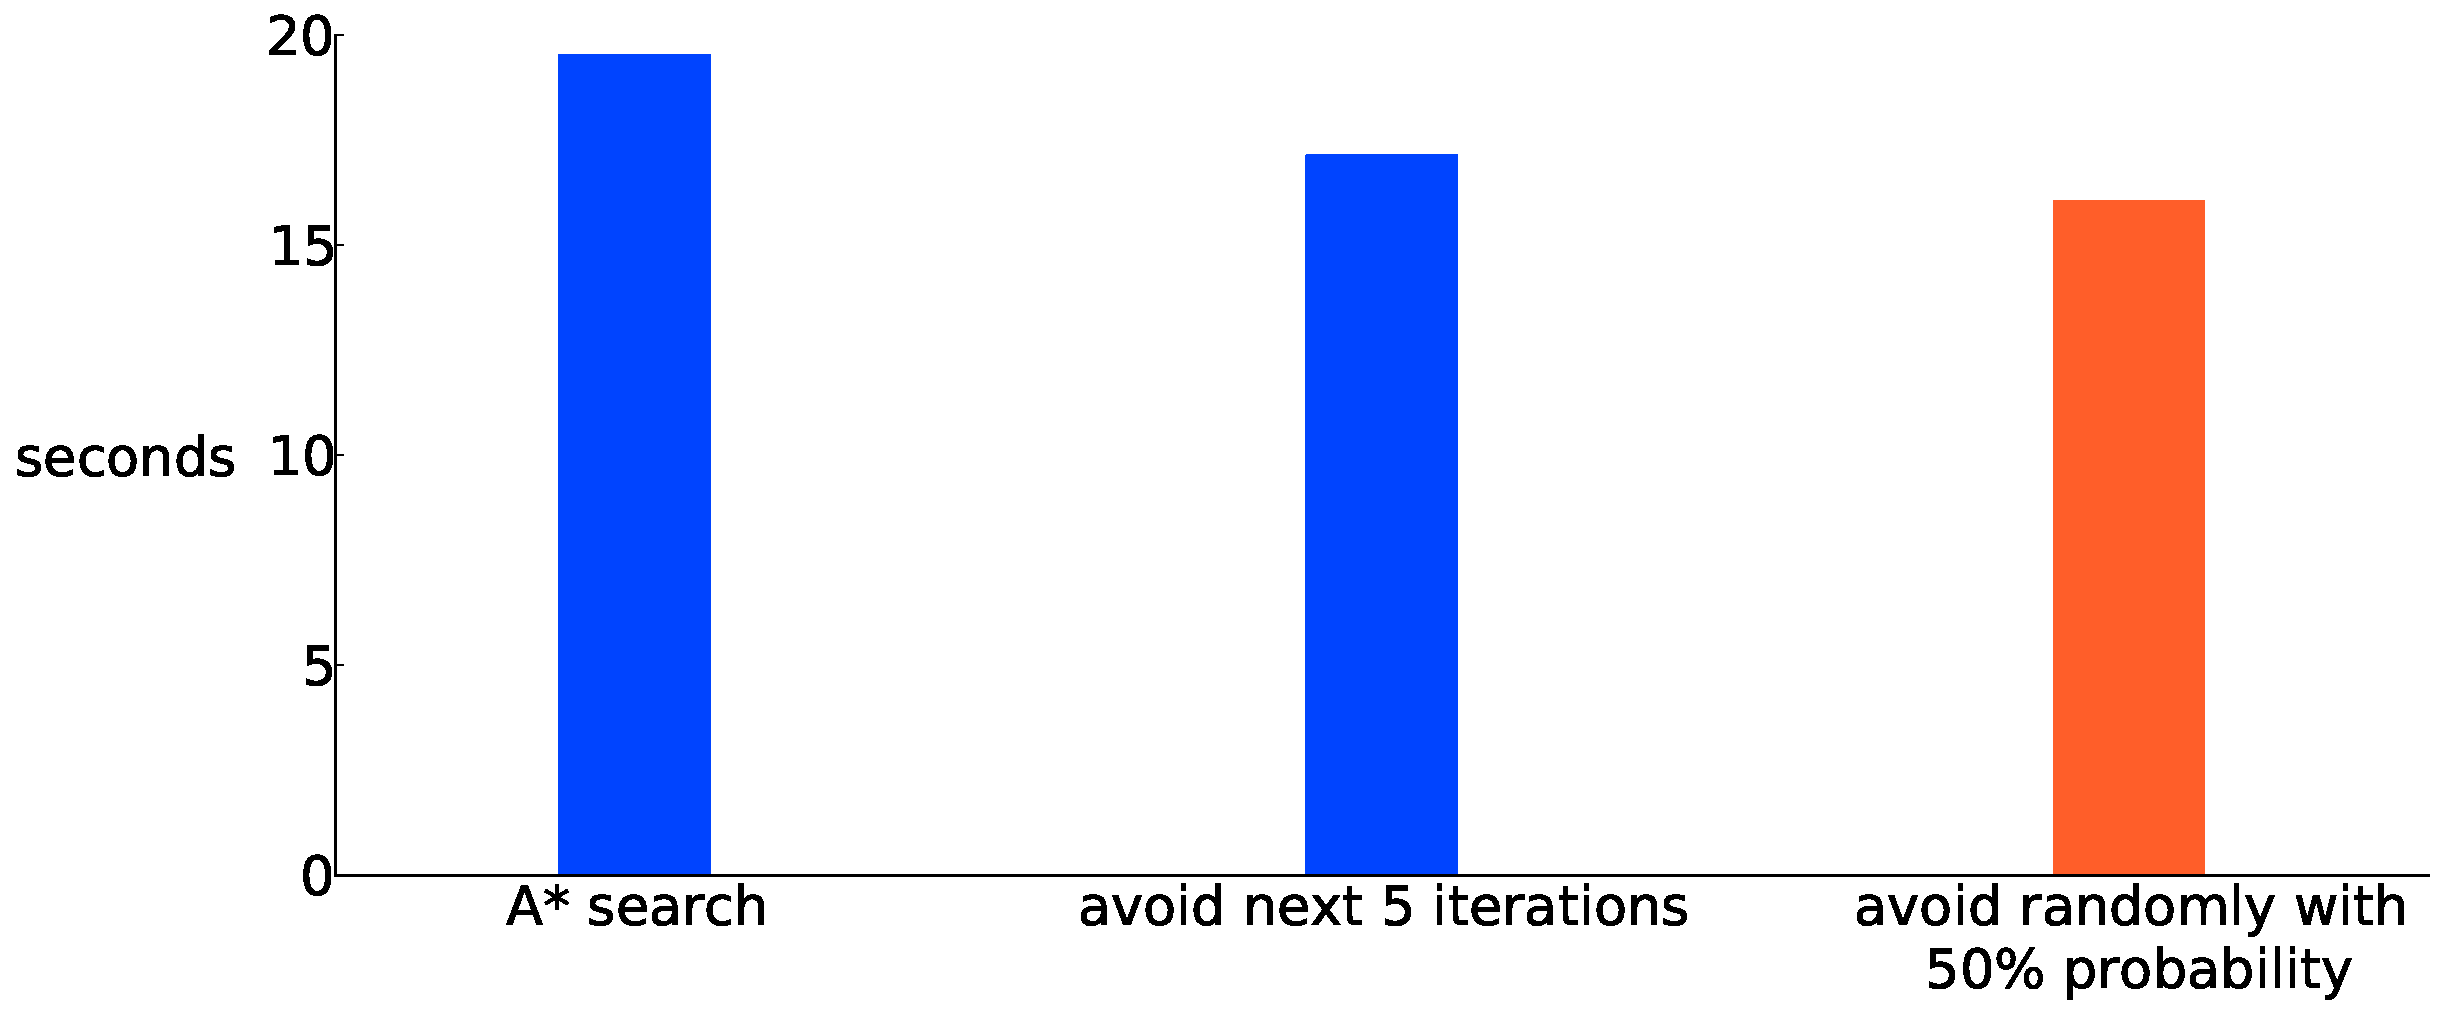
\includegraphics[width=\linewidth]{img/random_runtime}
            \end{figure}
        \end{block}
        \begin{block}{Conclusions}
            \begin{itemize}
                \itemsep.4em
                \item A* search algorithm using binary min-heap tree with random avoiding strategy has the \alert{best performance}
                \item \alert{30 times faster} than the existing implemented shortest path algorithm
             %   \item A \alert{30 times improvement} was observed compared to the existing implemented shortest path algorithm
            \end{itemize}
        \end{block}
    \end{column}
\end{columns}
\end{frame}

\end{document}
